% Version 2: Theme, Logo
\documentclass[11pt]{beamer}

\usetheme{Frankfurt}
\setbeamertemplate{navigation symbols}{}
\logo{
\includegraphics[height=0.5cm]{ssn.jpg}}
\title{Presentation in LaTeX}
\author{R S Milton}
\institute{
  Department of Computer Science\\
  SSN College of Engineering
}

\date{11 February 2017}

\begin{document}

\begin{frame}
  \titlepage
\end{frame}

\begin{frame}{Outline}
  \tableofcontents
\end{frame}


\section{Quick presentation}

\begin{frame}{Simple presentation}
  \begin{block}{Why LaTeX?}
    With LaTeX Beamer, we can make consistently looking presentation.
  \end{block}
  \begin{itemize}
  \item Use \texttt{beamer} class.
  \item Choose a theme.
  \item Otherwise, usual LaTeX.
  \end{itemize}
\end{frame}

\section{Blocks and columns}

\begin{frame}
  \frametitle{Simplicity}
  Use simple and direct words.
  \begin{block}{Herman Melville}
    A man of true science \ldots uses but few hard words, and
    those only when none other will answer his purpose; whereas
    the smatterer in science\ldots thinks, that by mouthing
    hard words, he proves that he understands hard things.
  \end{block}
  \begin{alertblock}{Herman Melville}
    A man of true science \ldots uses but few hard words, and
    those only when none other will answer his purpose.
  \end{alertblock}
  \begin{exampleblock}
    {Herman Melville}
    A man of true science \ldots uses but few hard words, and
    those only when none other will answer his purpose.
  \end{exampleblock}
\end{frame}

\begin{frame}
  \frametitle{Simplicity}
  Use simple and direct words.
  \begin{columns}
    \begin{column}{.45\textwidth}
      \begin{block}{}
        A man of true science \ldots uses but few hard words, and
        those only when none other will answer his purpose; whereas
        the smatterer in science\ldots thinks, that by mouthing hard
        words, he proves that he understands hard things.
      \end{block}
    \end{column}
    \begin{column}{.45\textwidth}
        A man of true science \ldots uses but few hard words,
        and those only when none other will answer his purpose;
        whereas the smatterer in science\ldots thinks, that by
        mouthing hard words, he proves that he understands hard
        things.
    \end{column}
  \end{columns}
\end{frame}

\begin{frame}
  \frametitle{What is Computer Science?}
  \begin{columns}
    \begin{column}{.5\textwidth}
    \begin{center}
      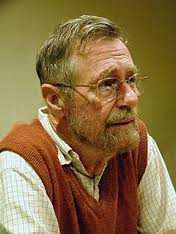
\includegraphics[scale=.5]{dijkstra.jpeg}
    \end{center}      
    \end{column}
    \begin{column}{.5\textwidth}
      \begin{exampleblock}{Dijkstra}
        Computer Science is no more about computers than
        astronomy is about telescopes or biology is about
        microscopes (E W Dijkstra).
      \end{exampleblock}
    \end{column}
  \end{columns}
\end{frame}


\section[Stepwise]{Stepwise}

\begin{frame}
  \frametitle{Pause}
  \begin{block}{Herman Melville}
    A man of true science \ldots \pause uses but few hard words,
    \pause and those only when none other will answer his
    purpose; \pause whereas the smatterer in science\ldots
    \pause thinks, that by mouthing hard words, he proves that
    he understands hard things.
  \end{block}
\end{frame}

\begin{frame}
  \frametitle{Pause}
  \begin{exampleblock}{Herman Melville}
    \onslide<1->{It is better to fail in originality, than to
      succeed in imitation. }%
    \onslide<3->{He who has never failed somewhere, that man
      can not be great. }%
    \onslide<2>{Failure is the true test of greatness.}
  \end{exampleblock}
\end{frame}


% \begin{frame}
%   \frametitle{Alternatives}
%   \begin{block}{Herman Melville}
%     \alt<2>{%
%       A man of true science \ldots uses but few hard words,
%       \pause and those only when none other will answer his
%       purpose; whereas the smatterer in science\ldots thinks,
%       that by mouthing hard words, he proves that he understands
%       hard things.}%
%     {%
%       It is better to fail in originality, than to succeed in
%       imitation. %
%       He who has never failed somewhere, that man can not be
%       great. %
%       Failure is the true test of greatness.}
%   \end{block}
  
% \end{frame}

\begin{frame}
  \frametitle{Stepwise revelation}
  \begin{columns}
    \begin{column}{.5\textwidth}
      \begin{block}{Just a block}
        \begin{itemize}
        \item<1-> First step.
        \item<2-> Second step.
        \item<3-> Third step.
        \end{itemize}
      \end{block}
    \end{column}
    \begin{column}{.5\textwidth}
      \begin{alertblock}{Another block}
        \begin{itemize}
        \item<1-> A step.
        \item<2-> B step.
        \item<3-> C step.
        \end{itemize}
      \end{alertblock}
    \end{column}
  \end{columns}
\end{frame}

\begin{frame}
  \frametitle{Stepwise revelation}
  \begin{minipage}{.45\linewidth}
    \begin{itemize}[<+->]
    \item First step.
    \item Second step.
    \item Third step.
    \end{itemize}
  \end{minipage}
  \begin{minipage}{.45\linewidth}
    \begin{itemize}[<+- | alert@+>]
    \item First step.
    \item Second step.
    \item Third step.
    \end{itemize}
  \end{minipage}
\end{frame}

\section{Graphics}
\begin{frame}
  \frametitle{Figure using tikz}
  \begin{center}
    A graphics will be placed here.
    % % \documentclass{article}

% \usepackage{tikz}
% \usetikzlibrary{arrows,shapes.geometric,shapes.symbols,scopes}

% \colorlet{DarkRed}{red!70!black}
% \colorlet{DarkBlue}{blue!70!black}
% \colorlet{DarkGreen}{green!50!black}

% \begin{document}

% Define block styles
\tikzstyle{block} = [rectangle, draw, draw=DarkBlue, inner
color=DarkBlue!0!white, outer color=DarkBlue!15!white,
text width=10em, thick,text centered, minimum height=2em] %

%\tikzstyle{line} = [draw, -latex']%
\tikzstyle{oval} = [rectangle, draw, draw=DarkGreen, fill=green!10, text width=10em, thick, text centered, rounded corners, minimum height=2em] %
\tikzstyle{arrow} = [thick,draw=DarkGreen,->,>=stealth]

\begin{tikzpicture}[node distance = 1.7cm, auto]
  % Place nodes
  \node [oval](in) {IE Extractions};
  \node [block, below of=in] (pc) {Predicate Counting};
  \node [block, below of=pc] (dg) {Graph Construction};
  \node [block, below of=dg] (gr) {Ground Rules Generation};
  \node [oval, below of=gr] (for) {First Order Rules};
  
  % Draw edges
  \draw [arrow] (in) -- (pc);
  \draw [arrow] (pc) -- (dg);
  \draw [arrow] (dg) -- (gr);
  \draw [arrow] (gr) -- (for);
\end{tikzpicture}
%\end{document}

  \end{center}
\end{frame}

\section{Table}

\begin{frame}{Course work}

  \begin{tabular}{lll}
    SNo & Code & Course Title\\\hline
    1 & CP7009 & Machine Learning Techniques\\
    2 & SE7003 & Machine Learning\\
    3 & MA7155 & Applied Probability and Statistics \\    
    4 & IF7203 & Data Warehousing and Data Mining \\
    5 & SE7204 & Big Data Analytics\\
    6 & CP7201 & Theoretical Foundations  of Computer Science\\
    7 & CP7024 & Information Retrieval Techniques \\
  \end{tabular} 
\end{frame}

\section{References}

\begin{frame}[allowframebreaks]
  \frametitle<presentation>{Reference}
  \small
  \begin{thebibliography}{10}
    \beamertemplatebookbibitems
  \bibitem{Marjan2009} Marjan Mernik, Dejan Hrncic, Barrett R. Bryant,
    Alan P. Sprague, Jeff Gray, Qichao Liu, Faizan Javed.
    \emph{Grammar Inference Algorithms and Applications in Software
      Engineering}, 978-1-4244-4221-8/09, IEEE, 2009.
  \bibitem{Colin2010} Colin de la Higuera.
    \emph{Grammatical Inference: Learning Automata and Grammars},
    Cambridge University Press, 2010.
 
    \beamertemplatearticlebibitems
    % Followed by interesting articles. Keep the list short.

  \bibitem{Arianna2011} Arianna D'Ulizia, Fernando Ferri, Patrizia
    Grifoni.
    \emph{A survey of grammatical inference methods for natural
      language learning},
    Artificial Intelligence Review, DOI 10.1007/s10462-010-9199-1,
    Springer, January 2011.
  \bibitem{Harald2013} Harald Lampesberger. 
    \emph{A Grammatical Inference Approach to Language-Based Anomaly
      Detection in XML},
    First Int Workshop on Emerging Cyberthreats and Countermeasures,
    Regensburg, Germany, September 2013.
  \end{thebibliography}
\end{frame}

\begin{frame}
  \vfill
  \begin{center}
    Questions?
  \end{center}
  \vfill
\end{frame}

\end{document}
